% Anhang
%

\chapter{Profiling}

For the profiling an own implementation is used based on wall clock timings.
The iteration loop \ref{ConnectAlg} is instrumented. An own implementation is
chosen to have full control about the disk and memory access of the profiler.
So io interruptions caused by the profiler are avoided.

Used code to get current timestamp:

\begin{lstlisting}
enum
{
	MICROSEC = (timeunit_t)1,
	MILLISEC = MICROSEC * 1000,
	SECONDS  = MILLISEC * 1000,
};

uint64_t get_timestamp ()
{
    struct timeval now;
    gettimeofday (&now, (struct timezone*)0);
    return  (uint64_t) now.tv_usec + 
            (uint64_t) now.tv_sec * SECONDS;
}
\end{lstlisting}

TraceLogger class handles the the measurements.
It generates buffers in the initialization and writes the measurements to file in the destruction.
For instrument a specific block or function in the algorithm \emph{start} and \emph{stop} function
\begin{lstlisting}
tracelogger.begin(0,"sort");
sort_function();
tracelogger.end(0,"sort");
\end{lstlisting}

The measured timings are written to an csv file, which has e.g. the following content:
\begin{lstlisting}
0;0;run;0;3793;116429658;
0;0;loadSynapses;0;2622330;4432049;
0;0;sort;0;4519751;5770458;
0;0;communicate;0;5770465;6366961;
\end{lstlisting}


Each row specifies one measurement. The columns contain the rank number, thread number, function name,
iteration number, start time and finish time respectively.

To get an overview the numbers are plotted in a raster plot.

\begin{figure}[ht!]
\centering
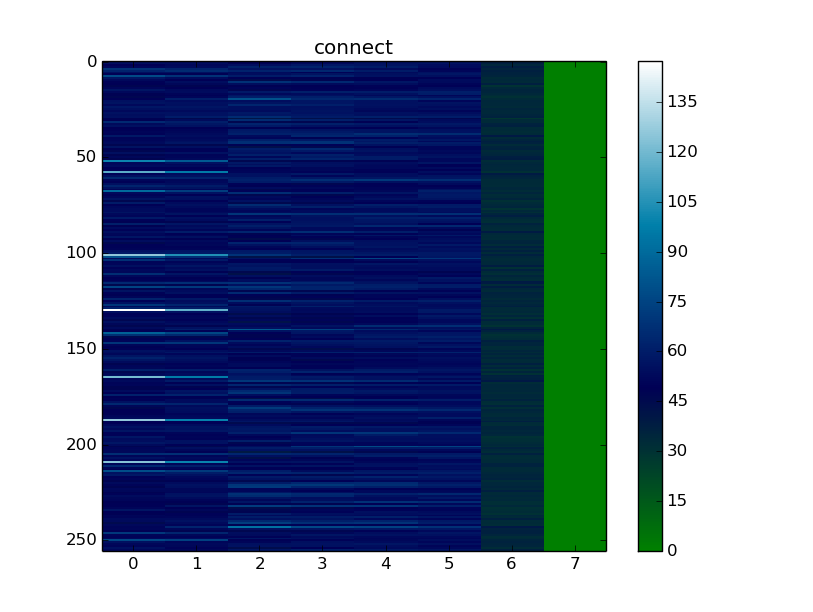
\includegraphics[scale=0.4]{pictures/1per300_tracefile_connect.png}
\caption{Visualized trace file}
\end{figure}

\chapter{Measure memory consumption}

\begin{lstlisting}


#include <stdio.h>
#include <spi/include/kernel/memory.h>

int getMemoryInformation(..)
{
  uint64_t shared, persist, heapavail, stackavail, stack, heap, guard, mmap;

  Kernel_GetMemorySize(KERNEL_MEMSIZE_SHARED, &shared);
  Kernel_GetMemorySize(KERNEL_MEMSIZE_PERSIST, &persist);
  Kernel_GetMemorySize(KERNEL_MEMSIZE_HEAPAVAIL, &heapavail);
  Kernel_GetMemorySize(KERNEL_MEMSIZE_STACKAVAIL, &stackavail);
  Kernel_GetMemorySize(KERNEL_MEMSIZE_STACK, &stack);
  Kernel_GetMemorySize(KERNEL_MEMSIZE_HEAP, &heap);
  Kernel_GetMemorySize(KERNEL_MEMSIZE_GUARD, &guard);
  Kernel_GetMemorySize(KERNEL_MEMSIZE_MMAP, &mmap);

  ..
}

\end{lstlisting}

\chapter{Mouse brain model standard use-case}
\label{ambmusecase}
In the thesis one virtual experiment is applied to the circuit inside of NEST.
It stimulates neurons which are related to the left whiskers.
Therefore the neuron hdf5 file contain a subnet dataset which contain a zero
for all neurons except of the related neurons. The related neurons have the entry 1.
A constant input current of 2500pA is set for these neurons.
A multimeter and spikedetector observes all neurons.
The circuit is simulated for 1000ms.

\chapter{HDF5 file of voxel list of long range generation}
\label{file:voxelinfo}
The list of processed voxels which is generated by the long range generation can be exported and imported
by the generation script. Therefore manipulation and debugging of the long range generation should be
simplified. The HDF5 file can be visualized and modified easily with Python. Further use-cases are 
splitting the generation in several files. Thus smaller synapse files can be generated.

HDF5 file properties



\chapter{Tools}

\section{h5py}
\section{numpy}
\section{matplotlib}
\section{Voxelize}
\section{Livre}
\section{Paraview}

